\documentclass{article}
\usepackage{verbatim}
\usepackage{hyperref}
\usepackage{fullpage}
\usepackage{amsmath}
\usepackage{graphicx}
\usepackage[shortlabels]{enumitem}

\title{Problem Set 1}
\begin{document}
\small
\date{Due date: March 2}
\author{Prof. Conlon}
\maketitle
Your answers should be produced in \LaTeX, and should include all relevant graph and code.  Code should be in the appropriate verbatim environment and properly documented. You are allowed to work in groups but you must turn in your own writeup. Submit your assignment via dropbox link to \href{mailto:cconlon@stern.nyu.edu}{cconlon@stern.nyu.edu}.

\section*{\normalsize Description of Nielsen Data}
This problem set uses simulated data that is made to look like responses of households to the Nielsen Consumer Panel Survey. An important feature of this dataset (and many other datasets) is that consumers report income in bands (between \$40,000 and \$50,000) rather than exact values. This can make estimating the overall distribution of income complicated. To make matters worse, there are also two regimes of coding income into bins. From 2006-2009 there are three extra bins for high earners. From 2010-onwards these bins are eliminated. Our goal is to construct a distribution of income for the provided panelists.\\

\noindent Each panelist is described by:
\begin{description}
\item[household\_code] a unique panelist identifier
\item[hh\_income] an income ``bin'' coded as below
\item[year\_regime] either `early' or `late' which denotes which bin assignments to use.
\item[number\_of\_hh] number of households in each ``bin''.
\end{description}

\begin{center}
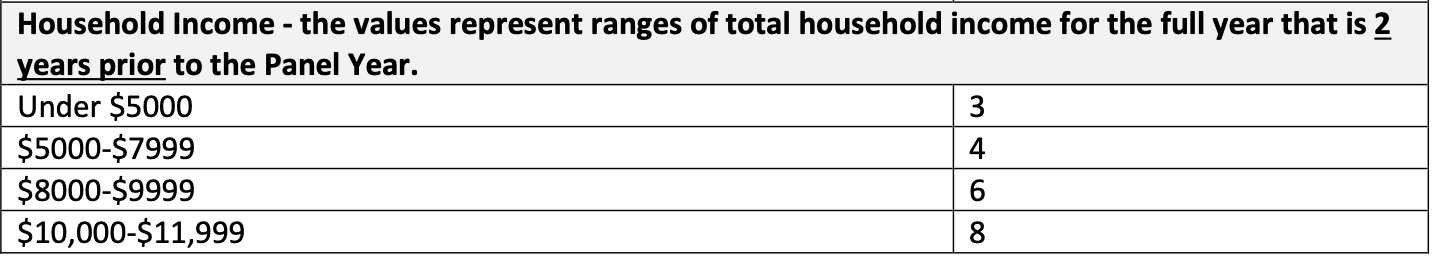
\includegraphics[width=4in]{./income_1.png}\\
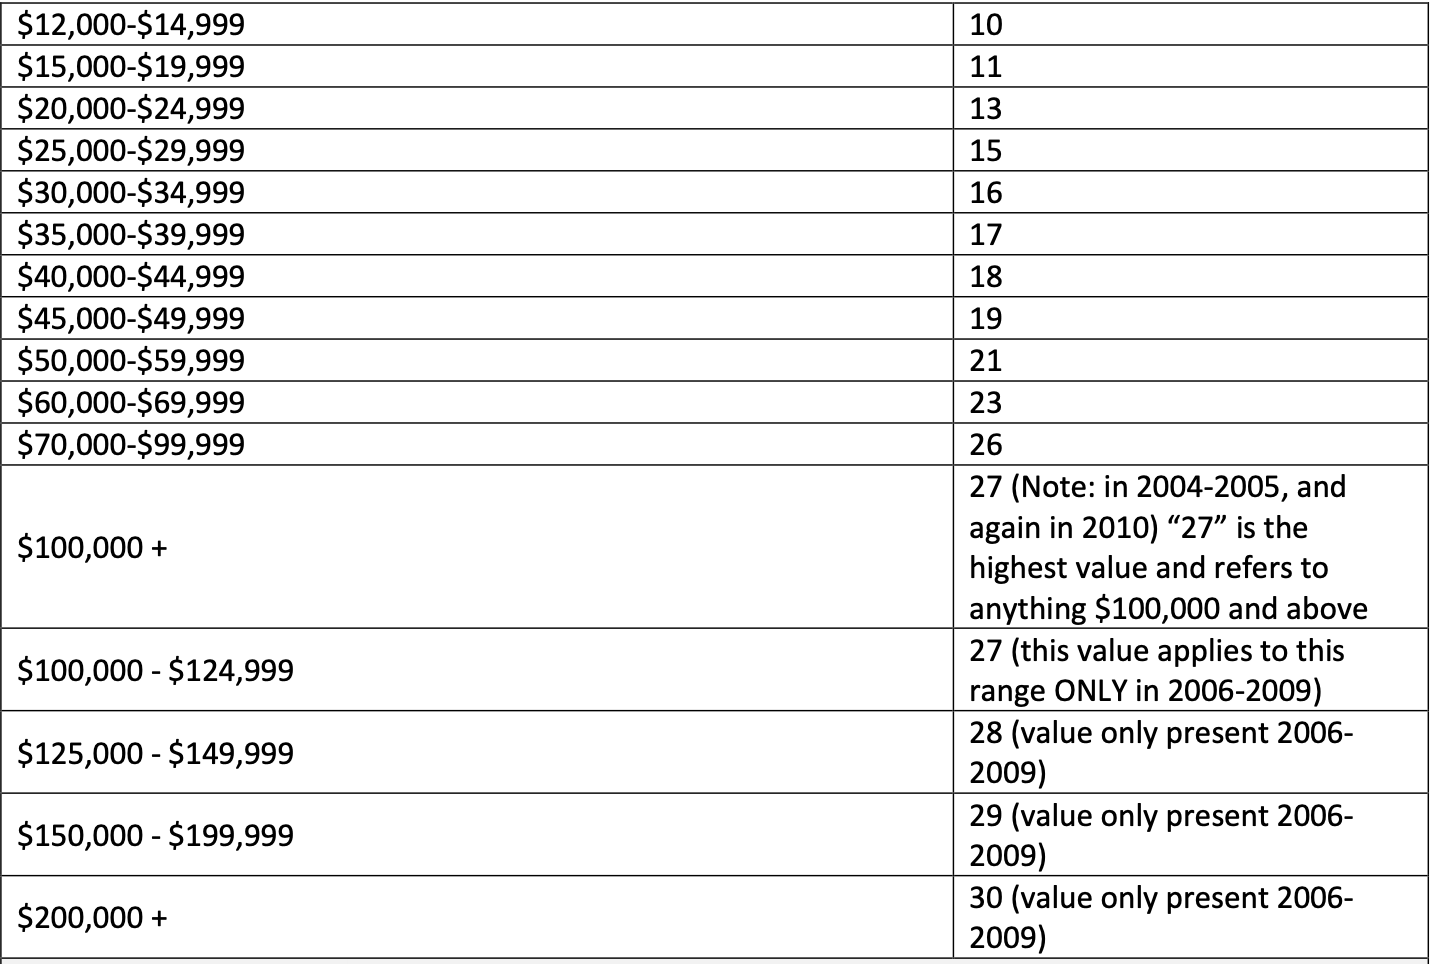
\includegraphics[width=4in]{./income_2.png}
\end{center}

\noindent For the first two method, we will want to estimate the lognormal parameters under three assumptions:
\begin{enumerate}[(a)]
\item Assuming each household earns the lowest income in each bin.
\item Assuming each household earns the highest income in each bin.
\item Assuming each household earns the mean income in each bin.
\end{enumerate}
Because income is top coded (b) and (c) are tricky. The goal here is to make reasonable assumptions, not ridiculous ones.

\section*{\normalsize Part 1: Method of Moments}
Let's begin by estimating a log-normal distribution of income. If income is distributed as $y_i  \sim LN (\mu,\sigma)$ then $\ln y_i \sim N(\mu,\sigma)$. We will start with a simple \textit{method of moments} estimator. Here the idea is to compute moments from our sample (means or variances $y_i$) and/or $\ln y_i$ and to use those to solve for parameters. You may want to look up the moments of the lognormal distribution on Wikipedia or in a textbook.

\begin{enumerate}
\item Estimate $(\mu,\sigma)$ working with $y_i$.
\item Estimate $(\mu,\sigma)$ working with $\ln y_i$.
\item Discuss how you would compute an estimate of the standard errors of $(\mu,\sigma)$. For extra credit: compute them.
\end{enumerate}

\section*{\normalsize Part 2: Maximum Likelihood}

Now let's consider a \textit{maximum likelihood estimator}. Again assume that the distribution of income is lognormal. 
\begin{enumerate}
\setcounter{enumi}{3}
\item Write the likelihood for the entire sample:  $Pr(y_1,\ldots,y_n | \mu, \sigma)$ or $Pr(\ln y_1,\ldots, \ln y_n | \mu, \sigma)$ \\ (Note: be careful that the coding of bins changes after 2010.)
\item Write the log-likelihood
\item Write the score of the log-likelihood for each $i$ and the overall gradient.
\item Estimate $(\mu,\sigma)$ correctly coding income before and after 2010.
\item Estimate the standard errors of $(\widehat{\mu}_{MLE},\widehat{\sigma}_{MLE})$ using the Fisher Information/Hessian Matrix.
\item Discuss your results so far. How sensitive are they to assumptions about the income bins? How sensitive are they to using the weighted vs. unweighted sample?
\end{enumerate}

\section*{\normalsize Part 3: Generalized Method of Moments}
Now let's write a GMM estimator that correctly handles the fact that we observe income in bins rather than directly observing income. Again we can assume that income is log-normally distributed and define the contribution of each observation as. The idea is to match the probability that an individual falls into a particular income bin in the data, to the probability that an individual falls in a particular income bin under the model:
\begin{align*}
g(y_i | \mu,\sigma) = Pr(40,000 \leq y_i \leq 44,999 | \mu,\sigma) -  \frac{1}{N}\sum_{i=1}^N I(40,000 \leq y_i \leq 44,999 | \mu,\sigma) 
\end{align*} 
\begin{itemize}
\item You will have at least one moment per bin.
\item You will also need to think about how you want to handle the fact that the income coding regime is not the same for the entire sample.
\end{itemize}
\begin{enumerate}
\setcounter{enumi}{9}
\item Write the Jacobian of the moment conditions with respect to the parameters $\frac{\partial g(y_i | \mu,\sigma)}{\partial \theta}$.
\item Estimate $(\mu,\sigma)$ using GMM. You will want to report the first stage estimates and the 2nd stage estimates.
\item Put all of your MoM, MLE, and GMM estimates into a table. Also compute the mean income in dollars and the 10th percentile and 90th percentile of the corresponding income distribution. How do they compare? How do standard errors compare?
\end{enumerate}


\section*{\normalsize Part 4: Nonparametric Estimates}
\begin{enumerate}
\setcounter{enumi}{12}
\item Plot a histogram of the income data. (It may be difficult to arrange the data into bins).
\item Plot your lognormal densities together on a single plot (Upper bound MLE, Lower Bound MLE, Mean MLE, and 2-step GMM estimates).
\item Estimate a kernel density plot for income (using the upper bound, the lower bound, and the mean of the bin) and compare that to your estimated lognormal densities.
\item Explain how the plots are similar and how they are different.
\end{enumerate}

\end{document}

